\section{Poisson Regression}

\subsection{Recommended References}
\begin{frame}{Recommended References}
	\begin{vfilleditems}
		\item \textcite{gelman2013bayesian} - Chapter 16: Generalized linear models
		\item \textcite{mcelreath2020statistical}:
		\begin{vfilleditems}
			\item Chapter 10: Big Entropy and the Generalized Linear Model
			\item Chapter 11, Section 11.2: Poisson regression
		\end{vfilleditems}
		\item \textcite{gelman2020regression} - Chapter 15, Section 15.2: Poisson and negative binomial regression
	\end{vfilleditems}
\end{frame}

\subsection{Count Data}
\begin{frame}{Count Data}
	Poisson regression is used when our dependent variable can only take \textbf{positive values},
	usually in the context of \textbf{count data}.
\end{frame}

\subsection{What is Poisson Regression?}
\begin{frame}{What is Poisson Regression?}
	Poisson regression behaves exactly like a linear model:
	it makes a prediction by simply computing a weighted sum of the
	independent variables $\mathbf{X}$ with the estimated coefficients $\boldsymbol{\beta}$:
	$\mathbf{y}$.
	But, different from linear regression,
	it outputs the \textbf{natural log} of $\mathbf{y}$:
	$$
		\log(\mathbf{y})= \alpha \cdot \beta_1 x_1 \cdot \beta_2 x_2 \cdot \ldots \cdot \beta_k x_k
	$$
	which is the same as:
	$$
		\mathbf{y} = e^{(\alpha + \beta_1 x_1 + \beta_2 x_2 + \ldots + \beta_k x_k)}
	$$
\end{frame}

\subsubsection{Exponential Function}
\begin{frame}{Exponential Function}
	The $e^x$ is called the exponential function
	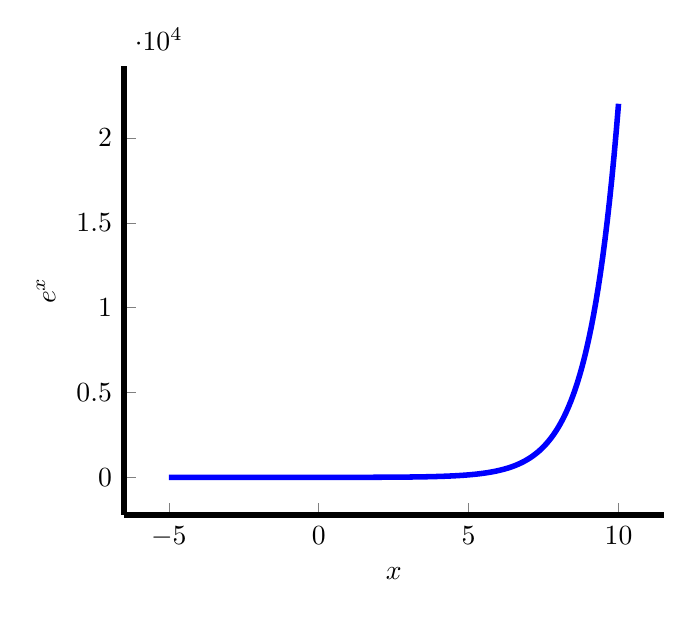
\begin{tikzpicture}
		\begin{axis}[every axis plot, line width=2pt,
				ylabel={$e^x$},
				xlabel={$x$},
				domain=-5:10,samples=200,
				axis x line*=bottom, % no box around the plot, only x and y axis
				axis y line*=left % the * suppresses the arrow tips
			]

			\addplot [blue] (x,{exp(x))});
		\end{axis}
	\end{tikzpicture}
\end{frame}

\subsection{Comparison with Linear Regression}
\begin{frame}{Comparison with Linear Regression}
	Linear regression has the following mathematical expression:
	\small
	$$
		\text{linear} = \alpha + \beta_1 x_1 + \beta_2 x_2 + \ldots + \beta_k x_k
	$$
	where:
	\begin{vfilleditems}
		\item \small $\alpha$ -- intercept.
		\item \small $\boldsymbol{\beta} = \beta_1, \beta_2, \dots, \beta_k$ -- independent variables' $x_1, x_2, \dots, x_k$ coefficients.
		\item \small $k$ -- number of independent variables.
	\end{vfilleditems}
	If you implement a small mathematical transformation,
	you'll have \textbf{Poisson regression}:
	\begin{vfilleditems}
		\item \small $\log{y} = e^{\text{Linear}} = e^{\alpha + \beta_1 x_1 + \beta_2 x_2 + \ldots + \beta_k x_k}$
	\end{vfilleditems}
\end{frame}

\subsection{Poisson Regression Specification}
\begin{frame}{Poisson Regression Specification}
	We can use Poisson regression if the dependent variable
	$\mathbf{y}$ has count data, i.e.,
	$\mathbf{y}$ only takes positive values.
	\textbf{Poisson likelihood function} uses an intercept $\alpha$ and
	coefficients $\boldsymbol{\beta}$,
	however these are ``exponentiated'' ($e^x$):
	$$
		\begin{aligned}
			\mathbf{y}     & \sim \text{Poisson}\left( e^{(\alpha +  \mathbf{X} \boldsymbol{\beta})} \right) \\
			\alpha             & \sim \text{Normal}(\mu_\alpha, \sigma_\alpha)                                   \\
			\boldsymbol{\beta} & \sim \text{Normal}(\mu_{\boldsymbol{\beta}}, \sigma_{\boldsymbol{\beta}})
		\end{aligned}
	$$
\end{frame}

\subsection{Interpreting the Coefficients}
\begin{frame}{Interpreting the Coefficients}
	When we see the Poisson regression specification,
	we realize that the coefficient interpretation requires a transformation.
	What we need to do is undo the logarithm transformation:
	$$
		\log^{-1}(x) = e^x
	$$
	So, we need to ``exponentiate'' the values of $\alpha$ and $\boldsymbol{\beta}$:
	$$
		\begin{aligned}
			\mathbf{y} & = e^{(\alpha +  \mathbf{X} \boldsymbol{\beta})}                                                                                                                                         \\
			               & = e^{\alpha} \cdot e^{ \left( X_{(1)} \cdot \beta_{(1)} \right) } \cdot e^{ \left( X_{(2)} \cdot \beta_{(2)} \right) } \cdot \dots \cdot e^{ \left( X_{(k)} \cdot \beta_{(k)} \right) }
		\end{aligned}
	$$
\end{frame}

\begin{frame}{Interpreting the Coefficients}
	Finally, notice that, when transformed,
	our dependent variables is no more a ``weighted sum of an intercept and
	independent variables'':
	$$
		\begin{aligned}
			\mathbf{y} & = e^{(\alpha +  \mathbf{X} \boldsymbol{\beta})}                                                                                                                                         \\
			               & = e^{\alpha} \cdot e^{ \left( X_{(1)} \cdot \beta_{(1)} \right) } \cdot e^{ \left( X_{(2)} \cdot \beta_{(2)} \right) } \cdot \dots \cdot e^{ \left( X_{(k)} \cdot \beta_{(k)} \right) }
		\end{aligned}
	$$
	It becomes a \textbf{``weighted product''}.
\end{frame}
